\newcommand{\PBoot}{\mathsf{PBoot}}
\newcommand{\XAsm}{\mathsf{XAsm}}

\section{Concurrent Machine Chain}
\label{sec:mach}

\ignore{
\paragraph{outline} 1) C-level vs assembly-level programming
2) layer refinement for composing multiple events?
3) spinlocks (ticket lock, MCS lock)
4)thread management
5) queuing locks
6) starvation-free condition variable
}

In this section, we introduce a realistic
concurrent multiprocessor machine model $\mach{x86mc}$,
and an assembly machine $\LAsm$ with a single active CPU
and suitable concurrent layer interfaces; then, we prove
refinement between these two machines.

\subsection{Concurrent hardware machine}
Our fine-grained multicore hardware $\mach{x86mc}$
is an \emph{abstract machine} (\cf Definition~\ref{def:mach}),
which allows arbitrary
interleavings at the level of \emph{assembly instructions}.
At each step, the hardware \emph{non-deterministically} chooses one CPU 
and executes the next assembly instruction on that CPU.


\paragraph{The machine state $\mach{x86mc}.S$} is a tuple $(c, f_\regs, m, a, l)$,
which consists of 
the current CPU $id$ $c$,
all CPUs' private states $f_\regs$
(\ie, a partial map from CPU $id$ to private state $\regs$),
a shared memory state $m$,
an abstract state $a$, and a global log $l$.
%The assembly language
%contains an extra register set component $regset$.
The private state $\regs$ consists of a CPU-local memory
(invisible to other CPUs) and a register set.

The global log $l$ 
is a list of events, which records all \emph{shared primitive calls} that affect more than
one CPU in the machine. Events generated by different CPUs are
interleaved in the log, following the actual chronological order of events.

The shared memory state  $m$ 
is \ignore{also  a sequence of
memory blocks, which are }shared among all CPUs.
Each shared memory location is associated
with a ``valid'' bit in the abstract state $a$, which can only be manipulated by 
two shared primitives called $\pull$ and $\push$. The $\pull$ operation
changes the bit from invalid to valid, after which shared memory accesses
can be performed. The $\push$ operation invalidates the bit
and records the shared memory updates to the log.
For example,
supposing
the last event in the log
is $``1.\push(i,x)"$
(\ie, CPU 1 pushed the value $x$ to the shared location $i$),
the memory accesses from CPU 0 to the shared location $i$
are shown as below:
\[
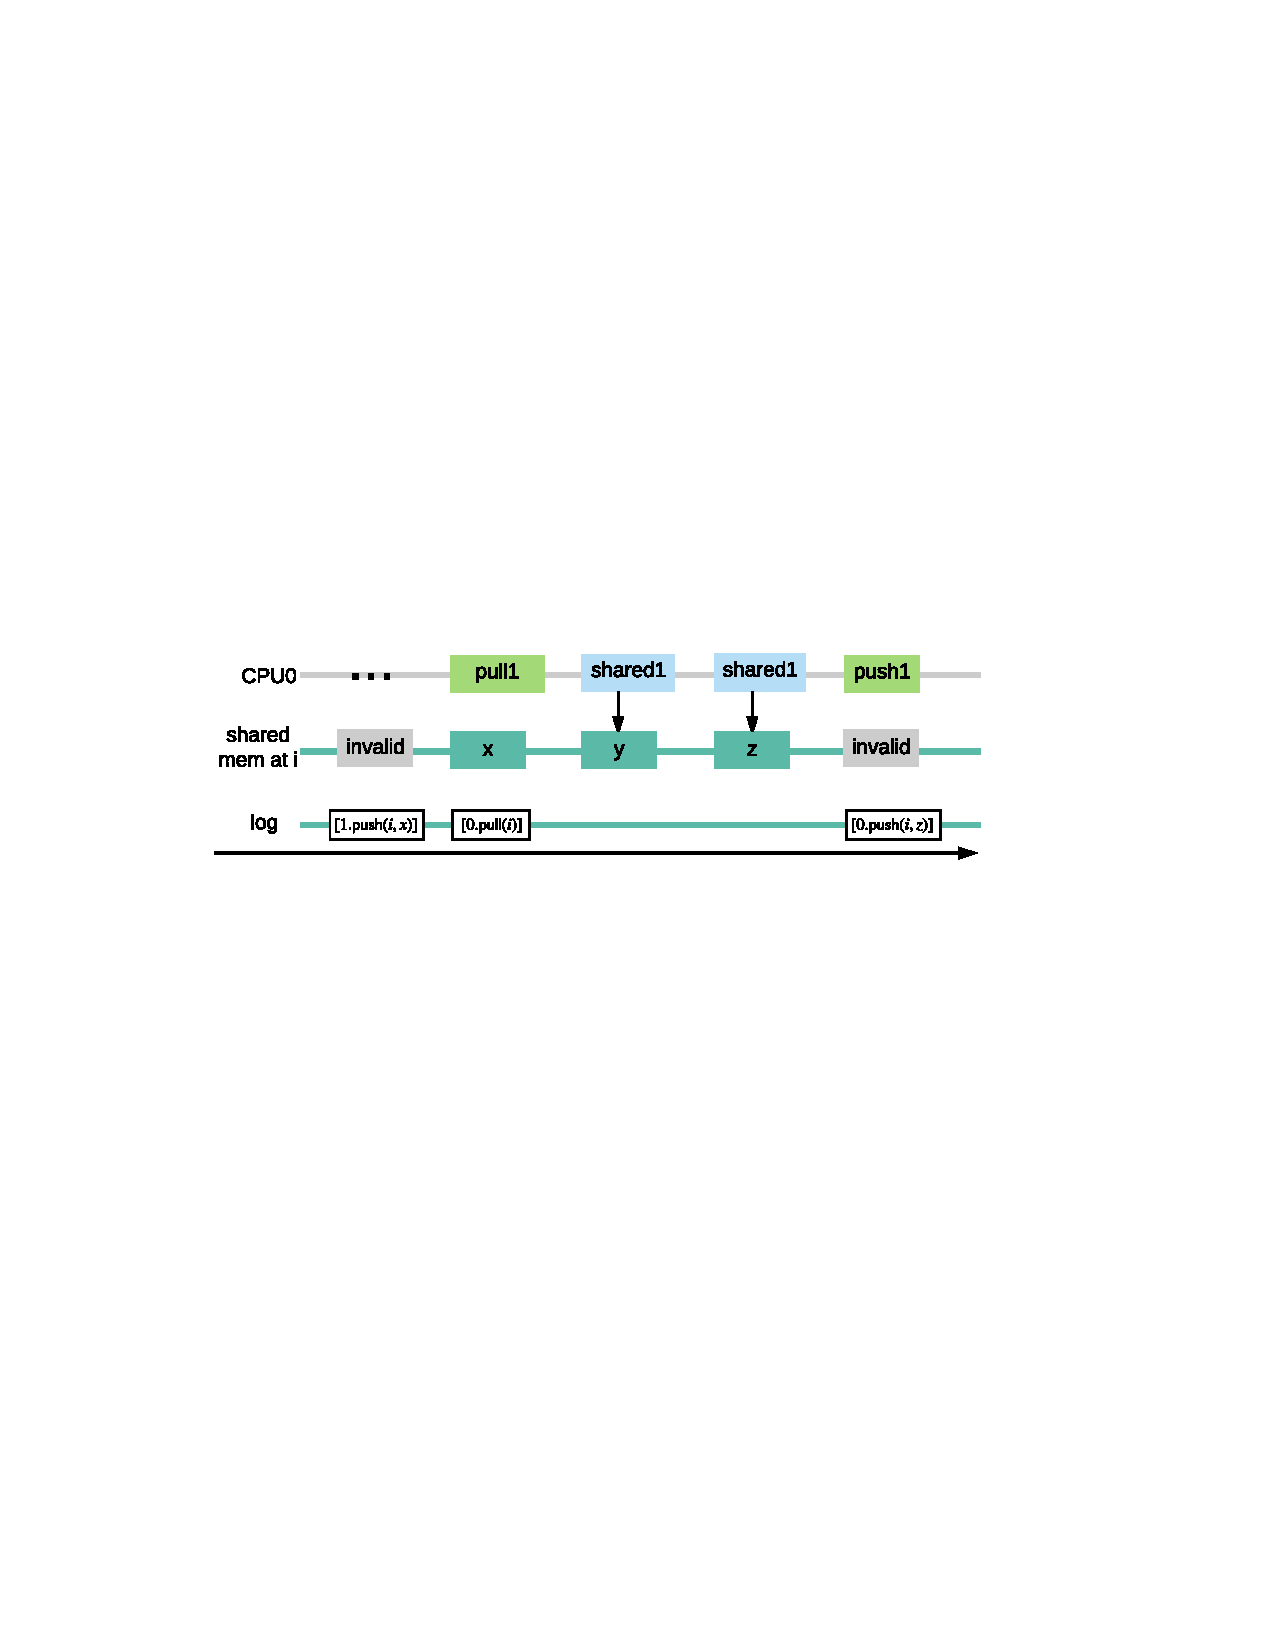
\includegraphics[scale=1]{figs/machine3}
\]
If a program tries to $\pull$ a shared memory location that is already valid,
this indicates a \emph{data race} and the machine gets \emph{stuck}.
One goal of concurrent program verification is to show
that a program is data-race free; in our setting, we accomplish 
this by showing that the program does not get stuck.

With this $\push/\pull$ model, shared memory accesses
can be treated as CPU-private executions,
whose effects to the whole machine
will be reflected by the following $\push$ operations. 

\paragraph{The transition relation $\mach{x86mc}.(\rightarrow)$}
consists of two types of transitions: 
\emph{program transitions} and \emph{hardware scheduling}, which can 
be nondeterministically interleaved.

\emph{Program transitions} can be of three types:
private transitions,
non-atomic shared transitions,
and atomic transitions.
Private transitions consist of
internal statements that only access
CPU-private memory
and  private primitive calls.
Non-atomic shared transitions
only include 
internal statements that access shared memory.
The first two types are ``local'', 
in that they can only access CPU-private 
state and the portion of shared memory marked as valid.
In both case, the global log $l$ will not be accessed.
Atomic transitions are
shared primitives calls, 
which will access shared objects
and provide the only means 
for accessing the global log and for generating events.
Both $\push$ and $\pull$ operations
are special shared primitive calls.
\ignore{
whose semantics is denoted
as the step relation $(args;s, res;s')$.
It says that starting from the state $s$ with the argument
$args$, the execution terminates with the state $s'$ and return
value $res$.}

\emph{A hardware scheduling transition} changes the
current CPU $id$ to some other $id$ 
and  can be arbitrarily interleaved with
program transitions.

This concurrent machine model $\mach{x86mc}$
reflects the nondeterministic concurrency features of 
multi-core hardware. 
One interleaving of an example program running on two CPUs
is:
\[
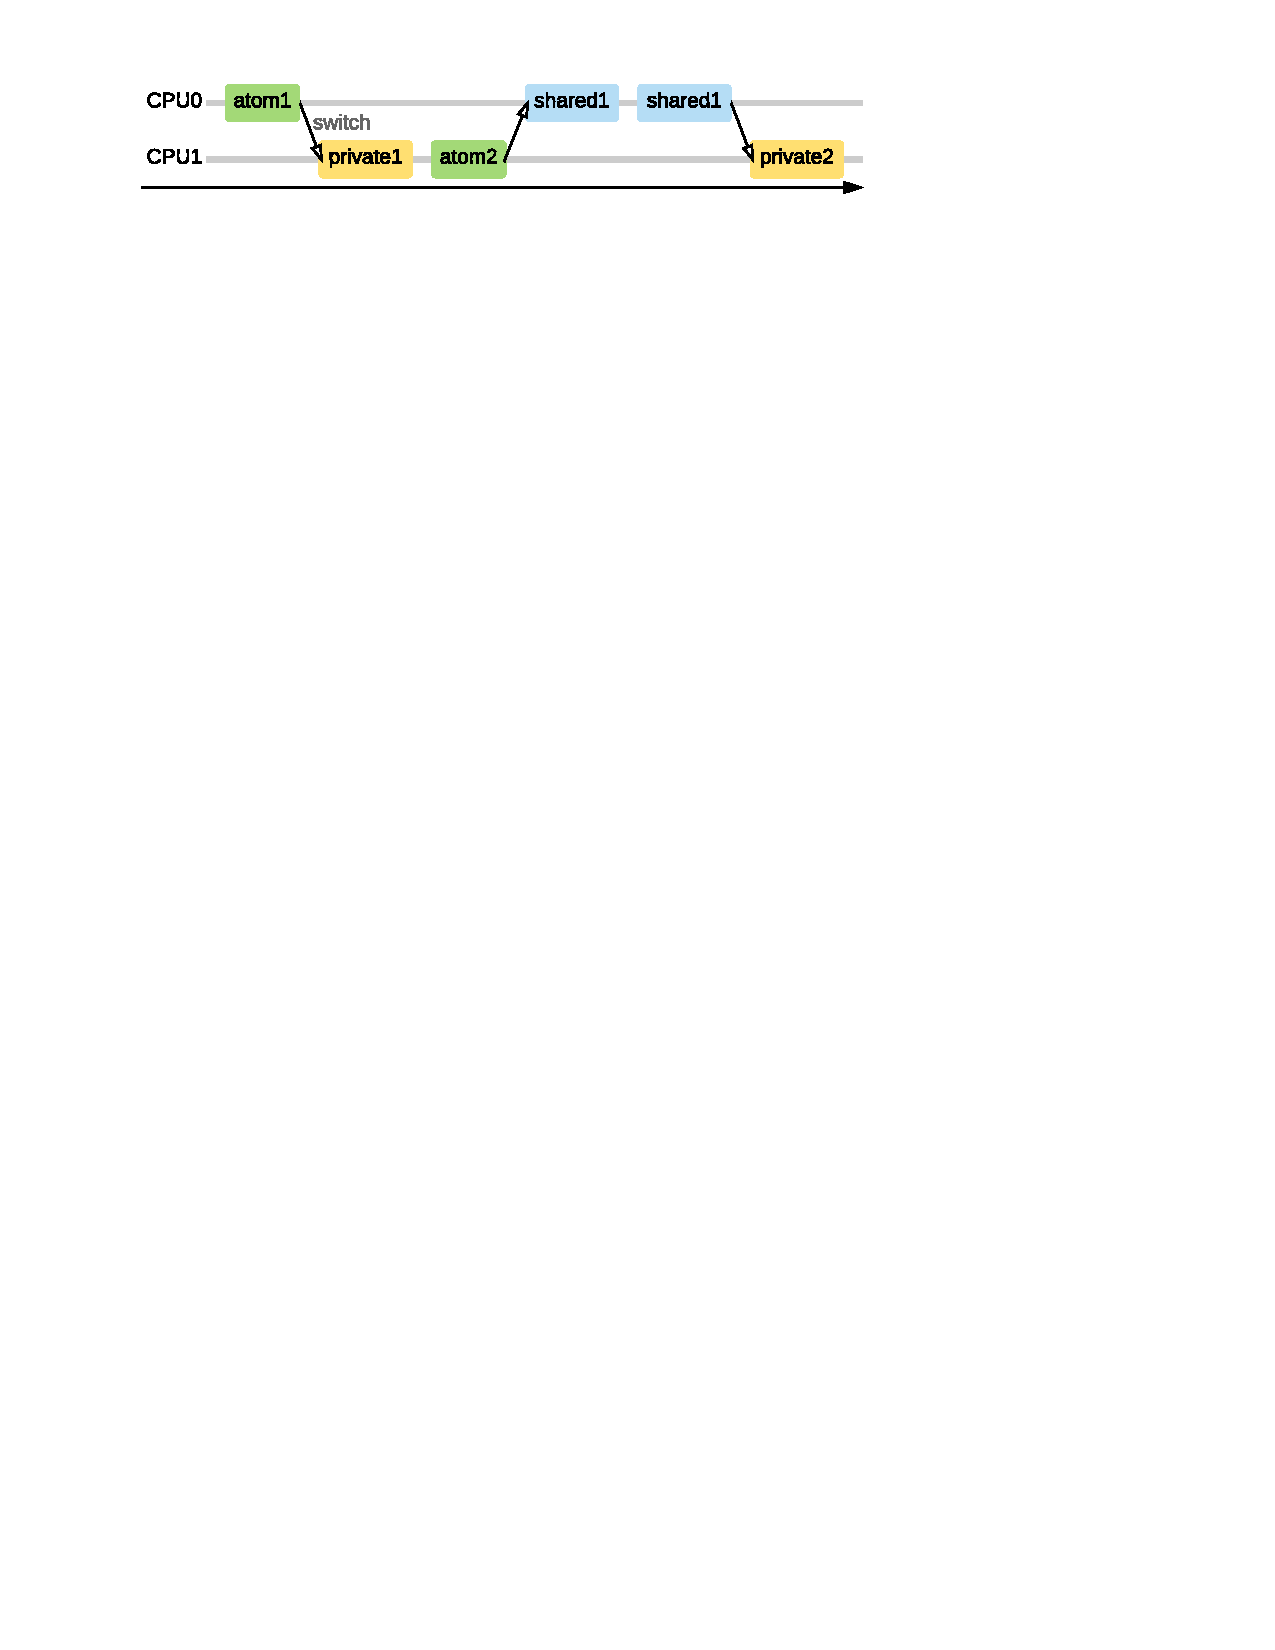
\includegraphics[scale=.93]{figs/machine1}
\]
Since only atomic transitions generate events,
this interleaving produces the logical log $(0.\mathsf{atom}_1)\cons
(1.\mathsf{atom}_2) \cons (0.\pull_1)
\cons (0.\push_1)$.

\paragraph{Sequential consistency}
The \push/\pull{} memory model
assumes that the memory of the multi-core hardware
is \emph{sequentially consistent}~\cite{lamport1979make}.
Previous work~\cite{steinke2004unified,
boudol2009relaxed,owens2009better} has shown that,
for data-race free programs,
multiprocessor executions 
can be modeled as a sequence of 
shared memory access events,
which is sequentially consistent.
Therefore, by showing that the \cCTOS{}
kernel will not go wrong over this \push/\pull{} memory model,
we have that \cCTOS{} is data-race free
and the sequential consistency assumption
is valid.

\subsection{Partial machine with hardware scheduler}
As a first step toward abstracting away the low-level details of
concurrent CPUs, we introduce a new partial machine ($\pmach{hs}$) configured
with a
\emph{hardware scheduler} ($\hardoracle$) that specifies a 
particular interleaving for an execution. 
This results in a deterministic machine model.
To take a program from $\mach{x86mc}$ and run it on top of $\pmach{hs}$,
we insert a  \emph{logical \intptext}
(denoted as ``$\intp$") before each assembly instruction.
Each switch point \intptext{}
yields to the hardware scheduler
and generates
a switch event
$c \switch hs$,
which is a \emph{local step} $\mach{hs}.\Delta$.
Then, the machine has to take
an \emph{environment step} to query the hardware scheduler
and get the CPU $id$ $c'$ to execute next.
This \emph{decision} made by $\hardoracle$ is stored in the 
log as a switch event $hs \switch c'$. 
The previous example on $\mach{x86mc}$
can be simulated by the following $\hardoracle$:\vspace{-5pt}
\[
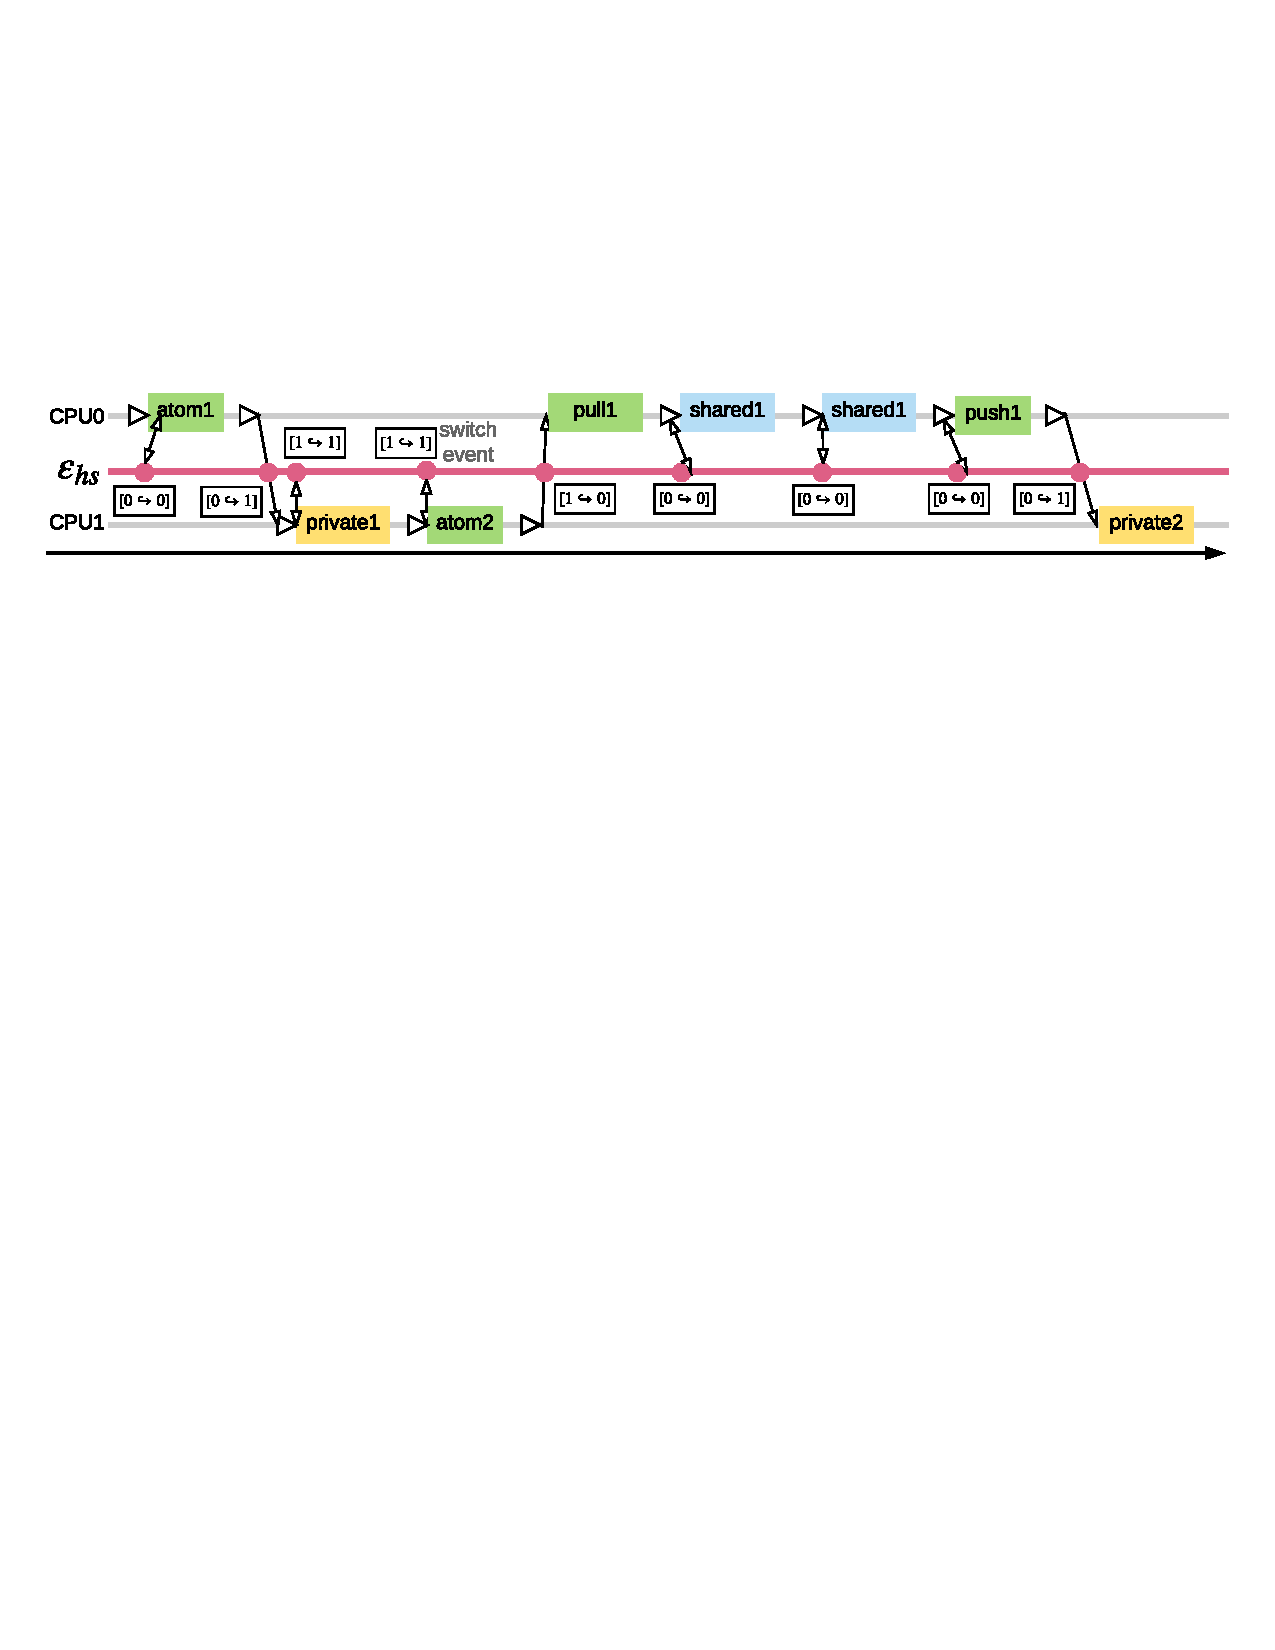
\includegraphics[scale=.75]{figs/machine2}
\]
\noindent
We write $(c \switch c')$
as an abbreviation of $(c \switch hs) \cons (hs \switch c')$.
Thus,
the log recorded by this execution is as follows:
\[
\begin{array}{l}
(0\switch 0) \cons (0.atom_1)
\cons (0\switch 1) \cons (1\switch 1)
\cons  (1\switch 1) \cons (1.atom_2)
\cons (1\switch 0) \\
\cons (0.\pull_1) 
\cons (0\switch 0)
\cons (0\switch 0)
\cons (0\switch 0)
\cons (0.\push_1) 
\cons ( 0\switch 1)
\end{array}
\]
\noindent
Note that this model is a special case of the partial
machine,
where the 
active set is the set of all CPUs,
and the environment is the hardware scheduler.
The \emph{rely} log invariant simply holds
on any log whose \emph{target} is $hs$:
\[\pmach{hs}.R := \{ l \in \Ev^* \ |\ \kw{target}(l) = hs \}\]
The \emph{guarantee} invariant states
two important properties:
\emph{data-race freedom}
and \emph{active consistency}.
The first property says
 that there is no
data race in the system,
\ie, there are no $\pull$ operations over $\code{valid}$
memory locations and every $\push$ operation
is done following its $\pull$ operation.
The second property simply
requires that all the events
are generated by the current active CPU or the hardware scheduler.
We write $\code{wf}$ for a predicate
over logs to state these two properties.
Thus, the guarantee invariant is shown below.
\[\pmach{hs}.G := \{ l \in \Ev^* \ |\ \kw{target}(l) \in \code{CPU\_set}
\land \code{wf}(l) \}\]
Any \emph{safe} execution of  local steps (\ie, $\pmach{hs}.\Delta$) results in a log $l \in \pmach{hs}.R \cup \pmach{hs}.G$.
Thus, since the hardware scheduler only returns switch events,
the result log of any environment step still satisfies
$\pmach{hs}.R \cup \pmach{hs}.G$ regardless
of the next CPU $id$ decided by the hardware scheduler.
To ensure the correctness of this machine,
we prove that $\mach{x86mc}$ \emph{refines} this
partial machine with hardware scheduler.

\begin{lemma}[Correctness of the hardware scheduler mode]
\[\mach{x86mc} \refines \bigcup_{\oracle_{hs}}{
\pmach{hs}\langle \oracle_{hs} \rangle}
\]\proof[Proof Sketch]
For any interleaved execution on $\mach{x86mc}$, we construct
a corresponding hardware scheduler on $\pmach{hs}$.
Thus, the log of $\mach{x86mc}$
is equal to the log of $\pmach{hs}$
by removing all the switch events.
 \label{lemma:pboot}
\end{lemma}


\subsection{Partial machine with environment context}

Although $\pmach{hs}$ is deterministic
with respect to a hardware scheduler,
it still does not have much support for CPU-local reasoning.
To support modular verification, 
we should provide a \emph{partial machine}
 to reason about programs on each CPU locally by specifying
expected behaviors of the context programs on other CPUs. Thus,
we can apply the linking theorems for the partial machine
 and 
 form a global
claim about the whole system. 
To this purpose, we introduce a partial
machine model $\mach{ec}$ that can be used to reason about the
programs running on a subset of CPUs, by
parametrizing the model over the behaviors of an \emph{environment context}
(\ie, the rest of the CPUs).

The active set $A$ of the partial machine  $\pmach{ec}$
is a local subset of CPUs,
and the context contains
both other CPUs and the hardware scheduler.
At each switch point,
the machine takes an environment step
to get the next CPU $id$ to execute.
If it yields a CPU outside the active set,
it will keep taking the environment step
to get the next event generated
by the context, until yielding back to an active CPU.

\paragraph{Environment context}
of $A$ in this machine model 
is denoted as $\ectxt{\pmach{ec}^A}$.
Each environment context $\oracle_{ec}\in\ectxt{\pmach{ec}^A}$
is a \emph{response function},
which takes the current log 
and returns an event from the context CPUs
or the hardware scheduler,
which is guaranteed to satisfy some invariant.
In other words, a response function simulates the observable behavior 
of the context CPUs and the potential interleaving, while the invariant states the assumptions being 
made over the context.
The execution of CPU 0 in the previous example can be simulated
with a $\oracle_{ec}\in\ectxt{\pmach{ec}^0}$.
\ignore{$\oracle_{\overline{\set{0}}}$
(\ie, $\oracle_{\set{1}}$, since there are only two CPUs).}
\[
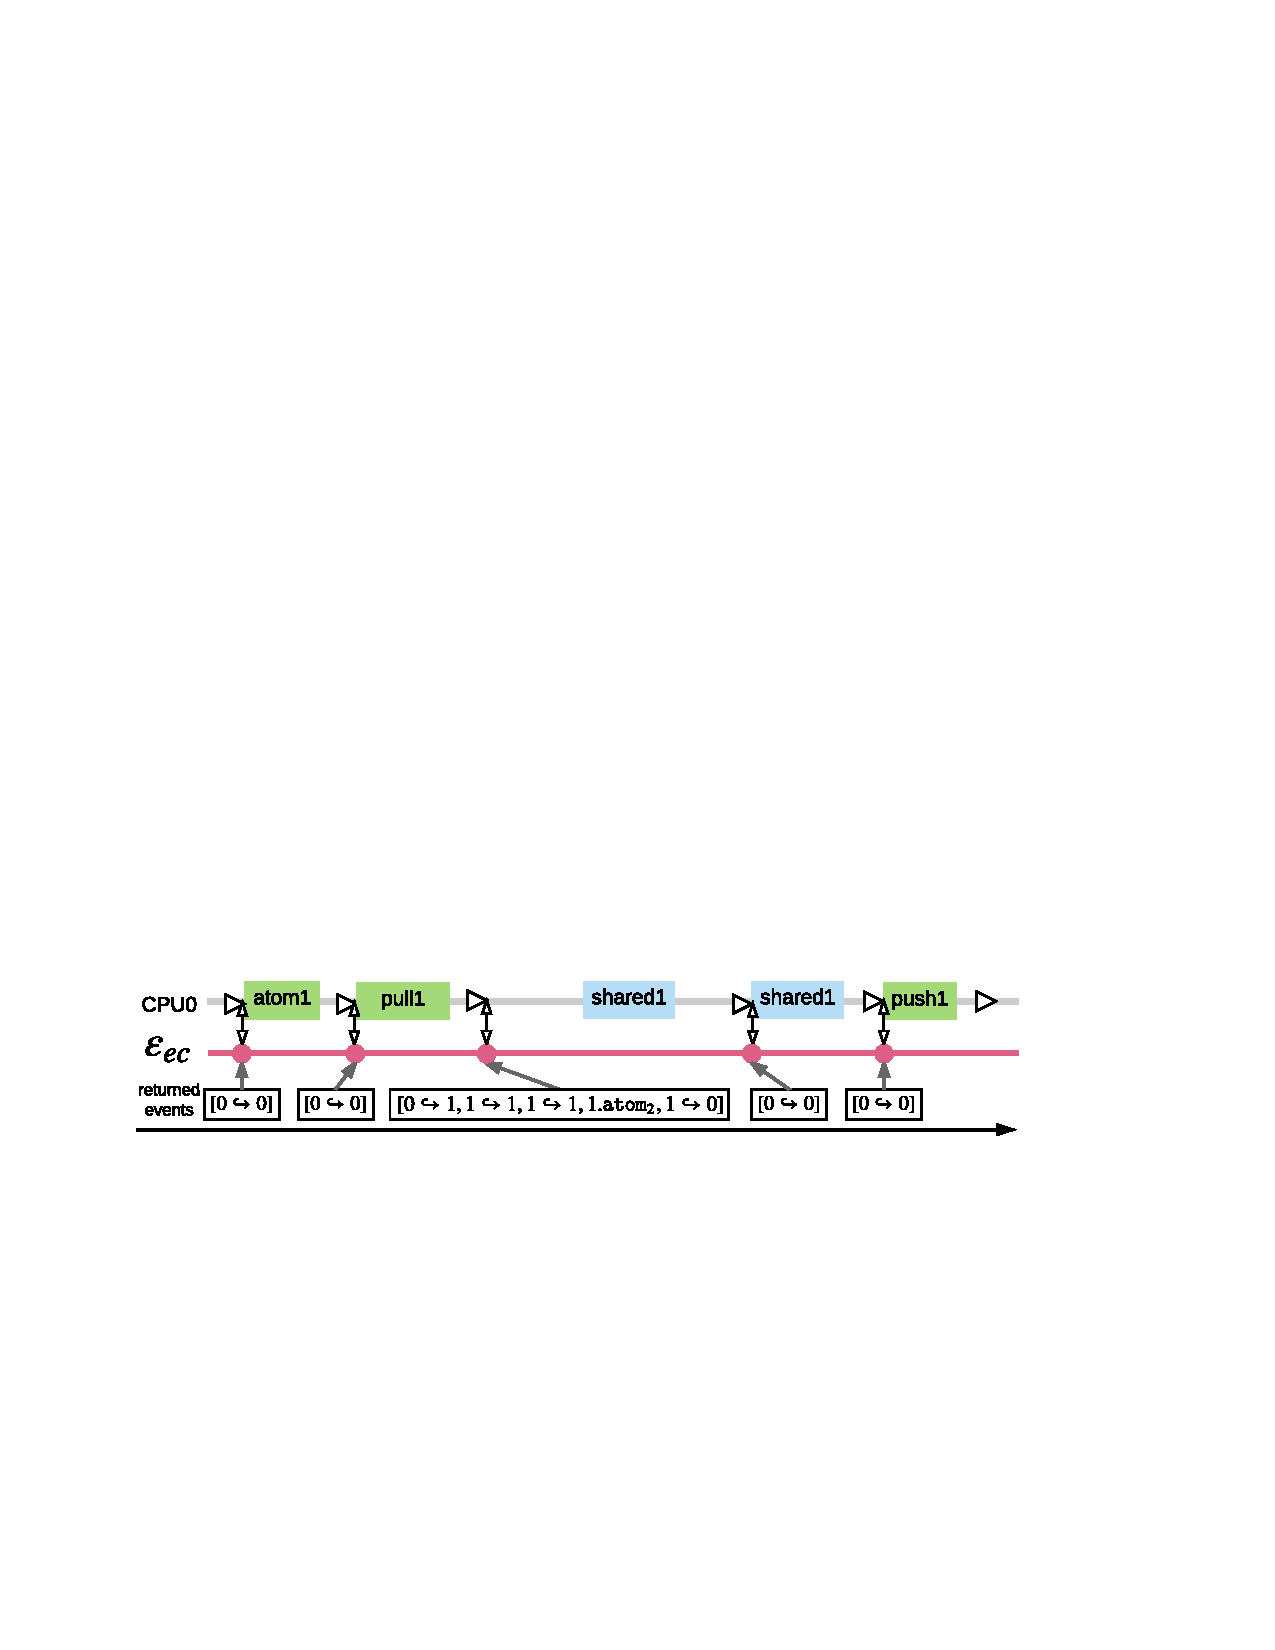
\includegraphics[scale=.9]{figs/machine4}
\]

\ignore{The environment context $\oracle_{\set{1}}$
generates the event list $[\event{0\switch 1},\event{1\switch 1},\event{1\switch 1}, \event{1.atom_2}, \event{1\switch 0}]$
at the third \intptext.}

\paragraph{Composition with environment context}
For the partial machine $\mach{ec}$,
both the rely and guarantee invariants
require the log to be well-formed.
\begin{align*}
\pmach{ec}^A.R := \{ l \in \Ev^* \ |\ \kw{target}(l) \not\in A
\land \code{well\_form}(l) \} \\
\pmach{ec}^A.G := \{ l \in \Ev^* \ |\ \kw{target}(l) \in A
\land \code{well\_form}(l) \}
\end{align*}
Therefore, for disjoint active sets $A_1$ and $A_2$,
the linking operator $\Join$ is well-defined 
(\cf Definition~\ref{def:link:partial})
and forms the linked partial machine:
\[\pmach{ec}^{A_1} \Join \pmach{ec}^{A_2}
\quad \text{ if } A_1 \cap A_2 = \emptyset\]

After composing the programs on all CPUs, the context CPU set becomes
empty, and the hardware scheduler is the only context.
Since we can prove that the log generated
by any safe execution on $\mach{hs}$
is well-formed,
the environment context is  is
reduced to the \emph{hardware scheduler}
$\oracle_{hs}$, which only generates the
switch events. In other words, by
showing that this \emph{composed machine} with the entire CPU set
is refined by $\pmach{hs}$, 
all the properties proved can be propagated down to the
multicore hardware model.

\begin{lemma}[Correctness of the environment context model]
\[\pmach{hs} \refines_\id \bigJoin_{c\in\comm{CPU\_set}}
\pmach{ec}^{c}\]
\end{lemma}


\subsection{CPU-local machine}
\label{subsec:spec:seq}
If we focus on a single active CPU $i$,
the partial machine $\pmach{ec}^i$ is like a \emph{local} machine
with an environment context representing all other CPUs
and the hardware scheduler. However,
in this model there is a {\intptext} before each instruction,
so program verification still needs to handle many unnecessary 
interleavings (\eg, the ones between private operations).
In this subsection, we introduce a CPU-local
machine model (denoted as $\pmach{loc}$) for a CPU $i$, in which {\intptext}s
only appear before shared atomic operations.
The {\intptext}s before shared or private operations
are removed via two steps: \emph{shuffling} and \emph{merging}.

\paragraph{Shuffling {\intptext}s}
In $\pmach{loc}$, we introduce a \emph{log cache}~--- for
the {\intptext}s before shared and private operations,
the query results from the environment context
are stored in a temporary log cache.
The cached events are applied to the logical log
just before the next shared atomic operation.
Thus, when we perform shared or private operations,
the observations of the environment context are delayed
until the next atomic operation.
This is valid because a shared operation can only be performed
when the current local copy of shared memory is valid, meaning that 
no other context program can interfere with the operation.

\paragraph{Merging {\intptext}s} Once the {\intptext}s are shuffled properly,
we merge all the adjacent {\intptext}s together.
When we merge {\intptext}s, we also need to merge 
the switch events generated by the environment context.
For example, the change of {\intptext}s for the previous example
on a CPU-local machine is as follows: 
\[
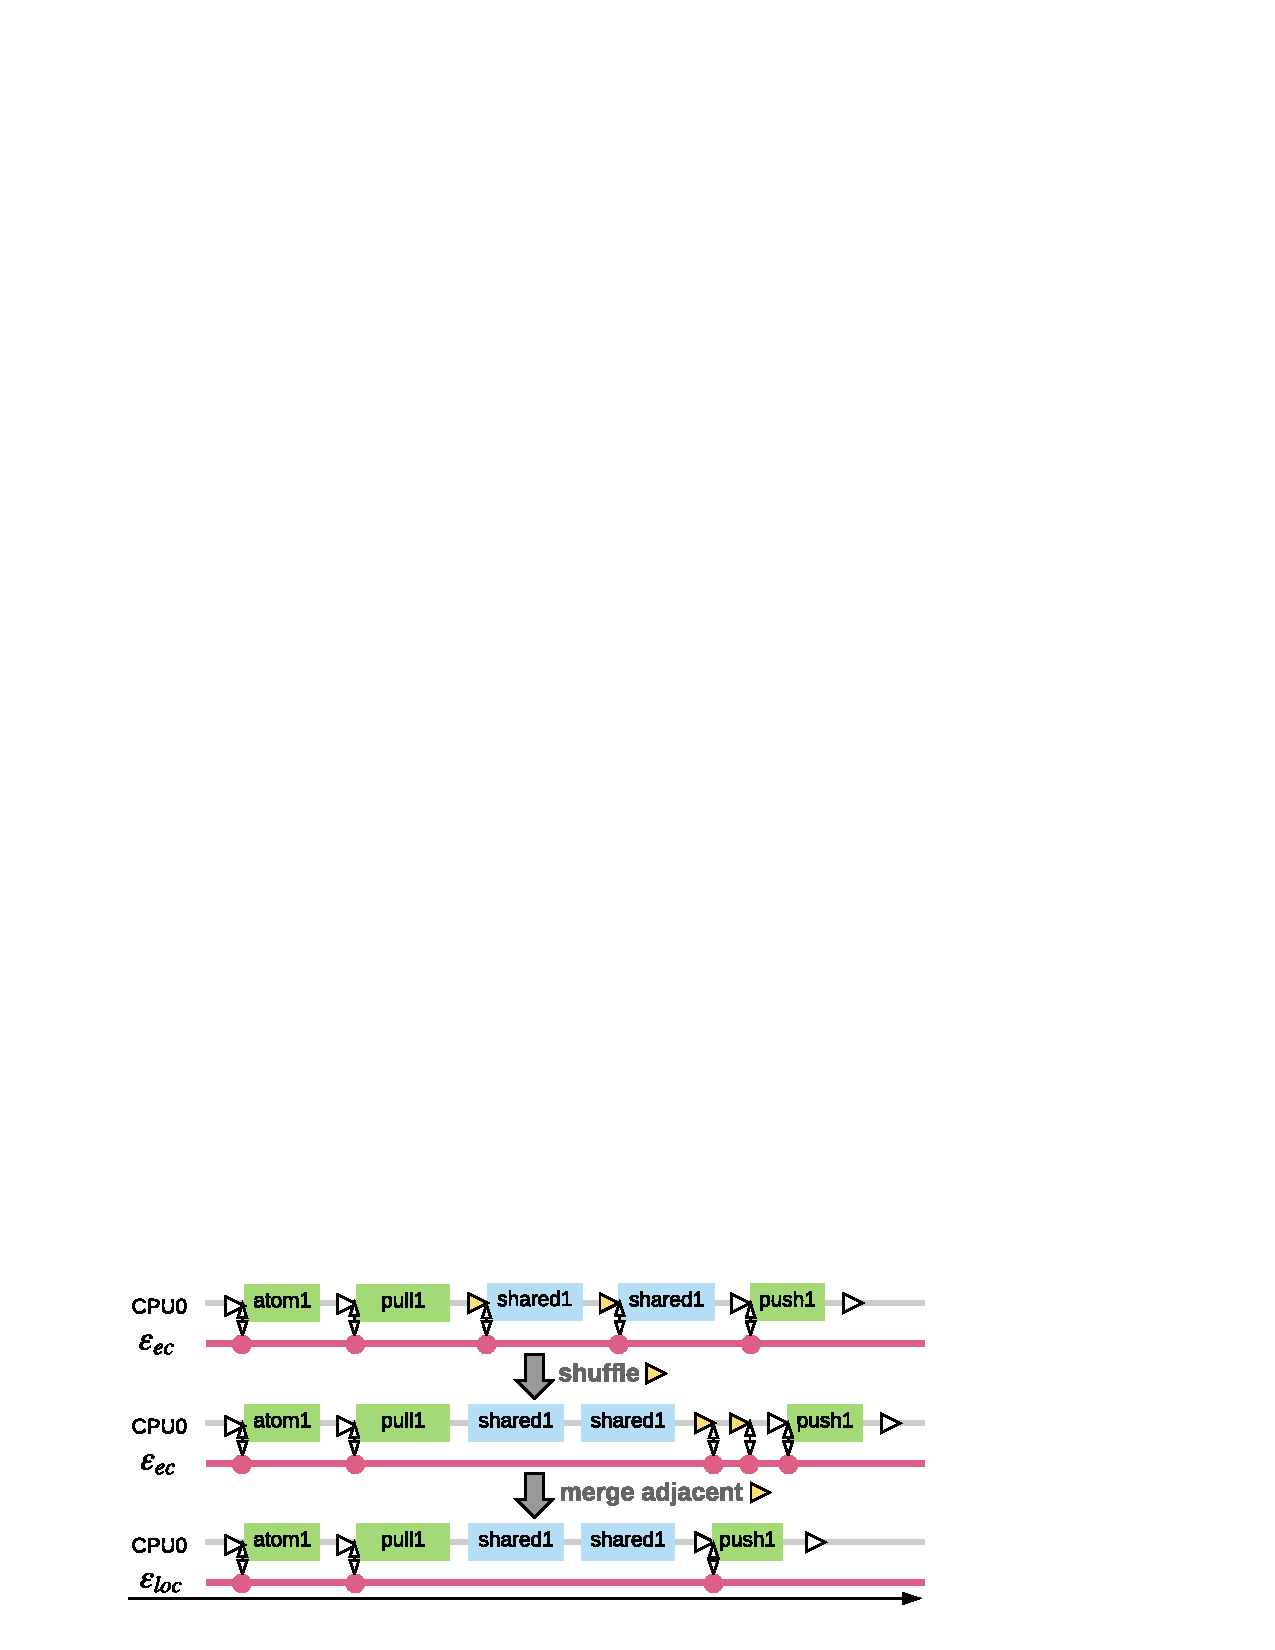
\includegraphics[scale=.9]{figs/machine5}
\]

\begin{lemma}[Correctness of CPU-local machine model]
\[\pmach{ec}^c \refines
\pmach{loc}^{c}\]

\ignore{
\[
\forall \oracle_{\overline{\set{i}}},
\exists \oracle'_{\overline{\set{i}}},
(\mach{pt},\oracle_{\overline{\set{i}}})_{\set{i}}
\machrel 
(\mach{loc},\oracle'_{\overline{\set{i}}})_{\set{i}}
\]
}
\ignore{\[
\begin{array}{l}
\forall P\ \oracle_{\overline{\set{i}}}\ \inv_{\set{i}},
\exists \oracle'_{\overline{\set{i}}},\\
\machbe{P}{\mach{pt}}{\oracle_{\overline{\set{i}}},  \inv_{\set{i}}}
\machrel 
\machbe{P}{\mach{loc}}{\oracle'_{\overline{\set{i}}}, \inv_{\set{i}}}
\end{array}
\]
\proof
Shuffling and merging {\intptext}s  are valid.
\qed}
\end{lemma}




\subsection{LAsm with concurrent layer interface}
\label{sec:con:lasm}

\ignore{
The Lemma~\ref{lemma:pboot} actually ``links'' $\PBoot$ with all
possible semantics for the hardware scheduler $hs$.}

%% Thanks to the Lemma~\ref{lemma:pboot}, the guarantees proved
%% over $\PBoot$ can be propagated down to the $\Mach_\boot$ level.

% TODO: This is wrong.
%% What's more, by the monotonicity lemma~\ref{lemma:mono},
%% we can build certified abstraction layers
%% with a single CPU $c$ on $\LAsm(L(c,\oracle))$, and compose the 
%% abstraction layers with the linking operator $\Join$.
%% In the rest of the paper, we will focus on this single-core
%% machine $\LAsm(L(c,\oracle))$.

\ignore{\paragraph{Single-core assembly machine $\LAsm(L(c,\oracle))$}}
The $\LAsm$ assembly machine model (\cf Section~\ref{sec:seq:lasm}) is
designed to ease sequential compositional reasoning. $\LAsm$ takes as
argument a sequential layer interface $L := (\abst, \primt_{\mathrm{ClightX}}, \primt_{\mathrm{LAsm}}, \invt, \mat)$
(\cf Definition~\ref{def:asm-layer}).
In the concurrent setting, we can reuse $\LAsm$ with an extended
notion of layer interface, \emph{concurrent layer interfaces}.

\begin{definition}[Multiprocessor layer interfaces]
A concurrent layer interface $L :=(\abst, \Ev, \primt_{\mathrm{ClightX}}, \primt_{\mathrm{LAsm}}, \invt, \mat)$ where 
$\Ev$ is the type for all possible events, and, for any CPU identifier $c$ and environment 
context $\oracle$, $\primt_{\mathrm{ClightX}}(c, \oracle)$ 
and $\primt_{\mathrm{LAsm}}(c, \oracle)$ are the sets of 
available C-style and assembly-style primitives. We then write $L(c, \oracle) = (\abst, \primt_{\mathrm{ClightX}}(c, \oracle), \primt_{\mathrm{LAsm}}(c, \oracle), \invt, \mat)$ to indicate the 
concurrent layer interface for processor $c$.
\end{definition}%
\noindent
Note $L[c]$ used in Section~\ref{sec:intro:layer}-\ref{sec:overview:concurrent}
can be viewed as a set of $L(c,\oracle)$ over any $\oracle$,
and the event type of $\oracle$ has to be consistent
with $L.\Ev$.

The $\LAsm(L(c, \oracle))$ machine state is thus defined as $\state:=(\regs, m, a, l)$,
where $\regs$ is the register set for CPU $c$,
$m$ is the memory state,
$a$ is the CPU-private abstract state,
and $l$ is the global log.
The big-step semantics of programs running on a single CPU is
almost the same with the one of LAsm,
shown in Section~\ref{sec:seq:lasm},
except that the machine state contains the log field $l$,
which will not be accessed by internal steps
and non-shared primitive calls.
We write $\oracle, c \vdash L.\primt_{\mathrm{ClightX}}(i) (args,m, a, l,res,m',a',l')$ to denote
the specification of the C-style primitive
with identifier $i$,
while we write $\oracle, c \vdash L.\primt_{\mathrm{LAsm}}(j) (\regs,m, a, l,\regs',m',a',l')$ to denote
the specification of the assembly-style primitive with identifier $j$.

Since there is a switch point $\intp$ 
in front of the shared primitive,
its semantics first query the environment context $\oracle$
with the current global log $l$
and update $l$ with the returned events generated by the environment.
We also \textbf{big-step} this query to simplify the representation,
which combines many actions.
First a switch event is
appended to the log $l$ indictating that we will interact with the
environment. Then the environment context $\oracle$ is queried
multiple times. Each time it returns an event from a CPU other than
$c$ we append that event to the log, and continue querying
$\oracle$. Finally $\oracle$ will yield back to $c$
(guaranteed by the \emph{fairness} of the hardware scheduler), and
the shared primitive call occurs.
The environment query is necessary before each shared primitive call because 
other CPUs must be given a chance to update shared state before the current 
CPU accesses it. 
\ignore{Note, however, that we do not need to worry about querying
the environment at internal statements and private primitives, since
the shared state cannot influence the behavior of these
transitions.} In the following, we will abuse notation and write
$l \cons \oracle(l)$ to mean the entire process of extending $l$ with
multiple events from other CPUs.
\ignore{which means that, starting from the log $l$, $\oracle(l)$ keeps
querying and appending events until the destination
is the current CPU $c$.}

In most cases, the execution of a primitive depends on what events have
been triggered at the switch point. 
For example, the $\pull$ primitive returns the
current state of the shared memory, which depends on what shared
memory updates from other CPUs are recorded in the global log.
To write the primitive specifications, we introduce an idiom of a
\textbf{replay function} $\replay$, which takes a
log as an argument and interprets it to calculate the ``current
state'' of the system after those events have happened. The
result of the replay function can be an arbitrary type, corresponding
to what kind of information is needed about the shared operations.

For example, the replay function $\replay_{\comm{get\_shared}}$
reconstructs the shared memory state from the given log.
It first retrieves the last shared memory
update to location $b$ from the log $l$. If the last update is
$c.\pull(b)$, it returns $(\any, \comm{invalid})$, where $\any$ denotes
any possible value. The shared memory state returned in this case
does not matter since the $\pull$ operation invalidates the corresponding
memory block. On the other hand, if the last update
is $c.\push(b,\comm{bl})$ for some byte list $\bytelist$,
it returns $(\comm{bl}, \comm{valid})$. 
If there is no $\push$ or $\pull$ event in the log, it returns
$(\any, \comm{valid})$. 
The rules for $\pull$ and $\push$ are defined as below:
\begin{small}
\begin{mathpar}
\inferrule{
   l_0 = l \cons \oracle(l) \\ 
  (\bytelist,  \comm{valid}) = \replay_{\comm{get\_shared}}(l_0, b) \\
  	m' = m \set{b: \bytelist} \\
  	a' = a \set{\perm{b}: \comm{valid}}  \\	
   l' = l_0 \cons c.\pull(b) \\ 
}{
 \oracle, c \vdash  \spec_{\pull}([b],\regs, m, a, l,\any, \regs,  m', a', l')
} 
\and
\inferrule{
  m(b) = \bytelist \\
  a.\perm{b} =  \comm{valid} \\
  a' = a \set{\perm{b}: \comm{invalid}} \\
  l' = l \cons  \oracle(l) \cons c.\push(b,\bytelist)   
}{
 \oracle, c \vdash  \spec_{\push}([b], \regs, m, a, l,\any, \regs, m, a', l')
}
\end{mathpar}
\vspace{-5pt}
\end{small}%

The $\pull$ operation requires the shared memory to be marked as valid
(after replaying the log). It first queries the environment context to update
the log, and then it updates the shared memory at location $b$ with the byte
list $\bytelist$ reconstructed from the log. This specification
captures the fact that the shared memory contents may be
modified by the environment context before the execution of
primitives. 
The $\push$ operation first gets the updated log from the environment context,
and then appends an event $c.\push(b,\bytelist)$ to the end of the log.
The operation is only defined when the permission bit is valid (\ie, the previous push
has already been pulled), and it invalidates the permission upon $\push$.

Let $L_\boot$ be the multiprocessor layer interface with the same abstract state, shared events, and primitives as in $\pmach{loc}$.
\ignore{
In general, $\LAsm(L(c, \oracle))$ is, however, not a partial machine.  For the
layer $L_0$ corresponding to primitives of $\mach{\boot}$, we have
constructed a partial machine $\XAsm(c)$ for a given core $c$ such
that:

\begin{lemma}
There exists a function $f$ such that, for any environment context $\oracle$: \[ \PBoot(\oracle) \refines \bigJoin_{c} \XAsm(c)(f(c, \oracle)) \]
\end{lemma}

\begin{lemma}
For any core $c$ and for any environment context $\oracle$: \[ \XAsm(c)(\oracle) \refines \LAsm(L_0(c, f(\oracle))) \]
\end{lemma}
\tahina{TODO: define $\XAsm$ and explain the proof}
}
Then,\ignore{For the layer $L_\boot$ corresponding to primitives of $\Mach_\boot$, } we
have proven that $\LAsm(L_\boot(c, \oracle))$ can be represented as a
partial machine, so that we can state and prove the following:
 \begin{lemma}
$ \forall \oracle.\ \pmach{loc}^c\langle \oracle \rangle \refines \LAsm(L_\boot(c, \oracle)) $
 \end{lemma}

\begin{figure}[t]\centering
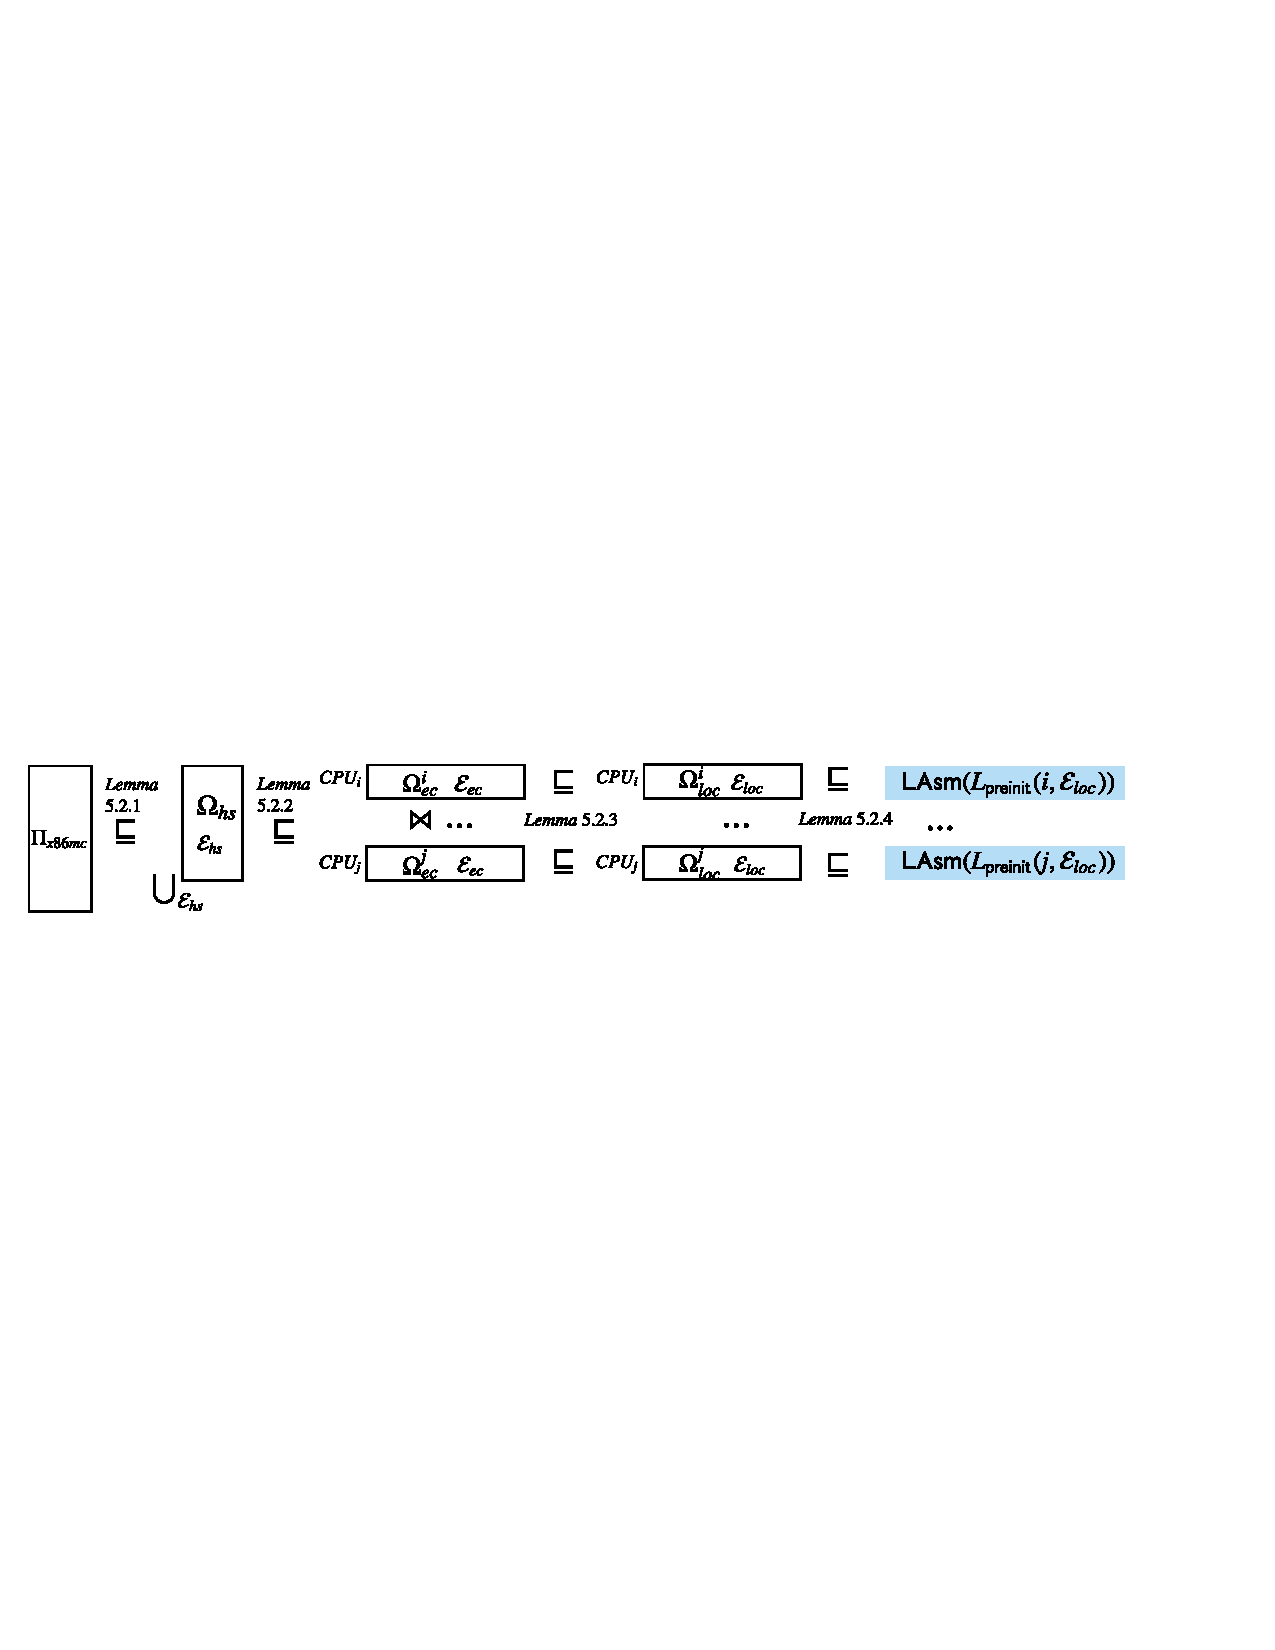
\includegraphics[scale=0.8]{figs/machine_chain}
\caption{The contextual refinement chain from multicore hardware model
$\mach{x86mc}$ to the LAsm machine
with single-core concurrent layer.}
\label{fig:spec:chain}
\hrulefill
\end{figure}

Finally, we obtain the refinement relation from the multicore
hardware model
to the single CPU LAsm machine model by composing
all of the refinement relations together (\cf Figure~\ref{fig:spec:chain}).
We introduce and verify the {\cCTOS} kernel on top of the
single CPU LAsm machine,
where the semantics of internal statements
and private primitives can be viewed as sequential,
and one only needs to consider concurrency
and interleaving at switch points (\ie, just before 
shared primitive calls).
The refinement proof guarantees that the proved properties can be
propagated down to the multicore hardware model $\mach{x86mc}$.


